\section{Lab Dokumentation}
Der Versuchsaufbau wird im TK-Labor C106 durchgeführt. Für den Aufbau sind die
folgenden IP-Adressen vorgesehen:

\begin{tabular}[t]{l l l l l}
\hline
Netz-ID & Router & Srv1 & Srv2 & Domain \\
\hline
\textcolor{red}{192.168.1.0} & 192.168.1.1 & 192.168.1.2 & 192.168.1.3 &
beta.tklabor.site \\ 
\textcolor{red}{192.168.1.16} & 192.168.1.17 & 192.168.1.18 & 192.168.1.19 &
antares.tklabor.site
\\
\textcolor{red}{192.168.1.32} & 192.168.1.33 & 192.168.1.34 & 192.168.1.35 &
orion.tklabor.site \\
\textcolor{red}{192.168.1.48} & 192.168.1.49 & 192.168.1.50 & 192.168.1.51 &
vogsphere.tklabor.site \\
\hline
\textcolor{red}{192.168.1.64} & 192.168.1.65 & 192.168.1.66 & 192.168.1.67 &
frogstar.tklabor.site \\
\textcolor{red}{192.168.1.80} & 192.168.1.81 & 192.168.1.82 & 192.168.1.83 &
epun.tklabor.site \\
\textcolor{red}{192.168.1.96} & 192.168.1.97 & 192.168.1.98 & 192.168.1.99 &
earth.tklabor.site \\
\textcolor{red}{192.168.1.112} & 192.168.1.113 & 192.168.1.114 & 192.168.1.115 &
earth2.tklabor.site \\
\hline
\textcolor{red}{192.168.1.128} & 192.168.1.129 & 192.168.1.130 & 192.168.1.131 &
fallia.tklabor.site \\
\textcolor{red}{192.168.1.144} & 192.168.1.145 & 192.168.1.146 & 192.168.1.147 &
magrathea.tklabor.site \\
\textcolor{red}{192.168.1.160} & 192.168.1.161 & 192.168.1.162 & 192.168.1.163 &
lamuella.tklabor.site \\
\textcolor{red}{192.168.1.176} & 192.168.1.177 & 192.168.1.178 & 192.168.1.179 &
kria.tklabor.site \\
\hline
\textcolor{red}{192.168.1.192} & 192.168.1.193 & 192.168.1.194 & 192.168.1.195 &
zarss.tklabor.site \\
\textcolor{red}{192.168.1.208} & 192.168.1.209 & 192.168.1.210 & 192.168.1.211 &
rupert.tklabor.site \\
\textcolor{red}{192.168.1.224} & 192.168.1.225 & 192.168.1.226 & 192.168.1.227 &
eadrax.tklabor.site \\
\textcolor{red}{192.168.1.240} & 192.168.1.241 & 192.168.1.242 & 192.168.1.243 &
thesun.tklabor.site \\
\hline
\end{tabular}
\newline
\newline
Die entsprechenden Adressbereiche werden für die Gruppen wie folgt aufgeteilt:
\begin{figure}[H]
\begin{center}
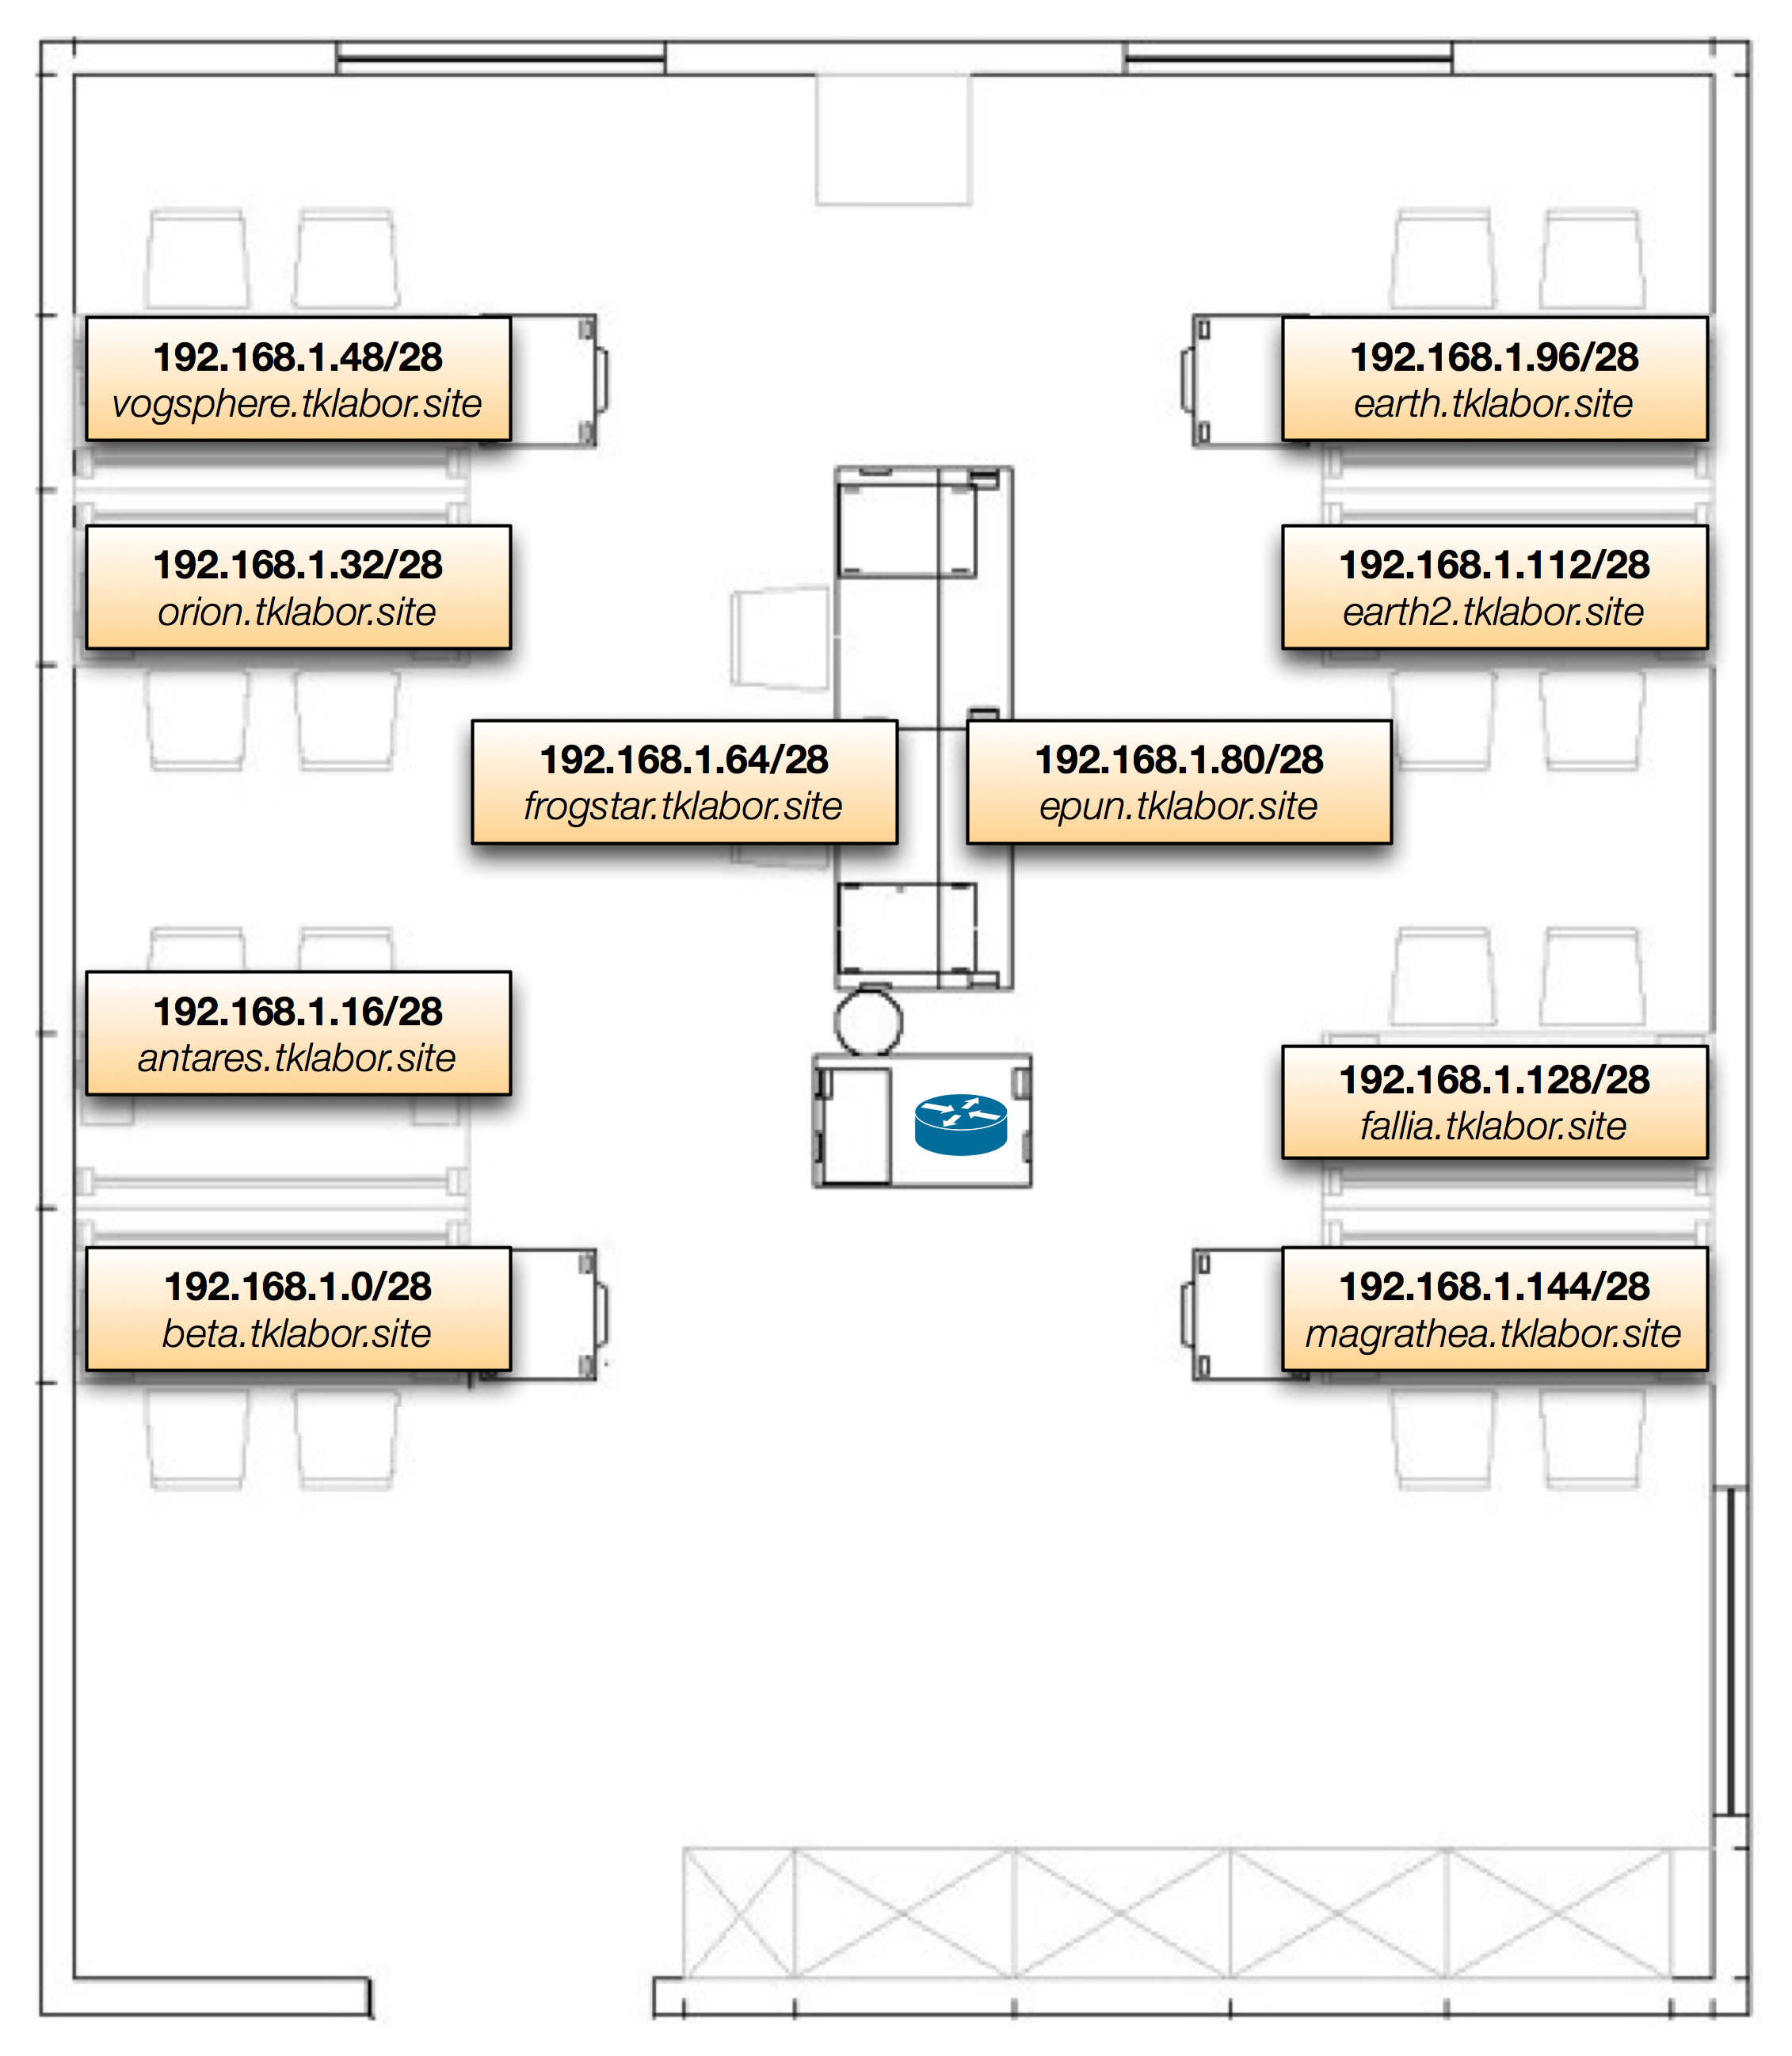
\includegraphics[width=0.75\textwidth]{images/lab-aufbau.png}
\end{center}
\end{figure}